\subsection{Map}

Data is displayed on a map using \texttt{mapbox-gl-js}\footnote{\url{https://docs.mapbox.com/mapbox-gl-js/api/}}, which allows for easy consumption of GeoJSON data, as well as highly customisable styling and complex data visualisation due to the use of vector data and arbitrary WebGL layers. The map uses a light, low contrast style \texttt{Mapbox Light}\footnote{\url{https://www.mapbox.com/maps/light-dark/}} which provides a simple, distraction-free background on which to display data, allowing the data visualisation to be the standout element.

\subsection{Heatmaps}

Tweet data was displayed in two ways: a heatmap at distant zooms, to provide an overview of tweet density; and individual interactable tweets at close zooms, to allow direct inspection of the data. Due to the data-driven API provided by \texttt{mapbox-gl-js}, displaying the tweets as a heatmap and switching between visualisation types is extremely simple.

AURIN data is displayed as a 3-dimensional heatmap, where colour of regions is complemented by a vertical region projection, such that regions with higher poor health scores are more visually prominent in multiple dimensions. This uses a data-driven \texttt{fill-extrusion} layer to project the regions vertically, to a height proportional to their scores. Height is slightly exaggerated for regions with higher scores using an exponential curve, in order to provide slightly better visual distinction.

\begin{figure}[H]
    \centering
    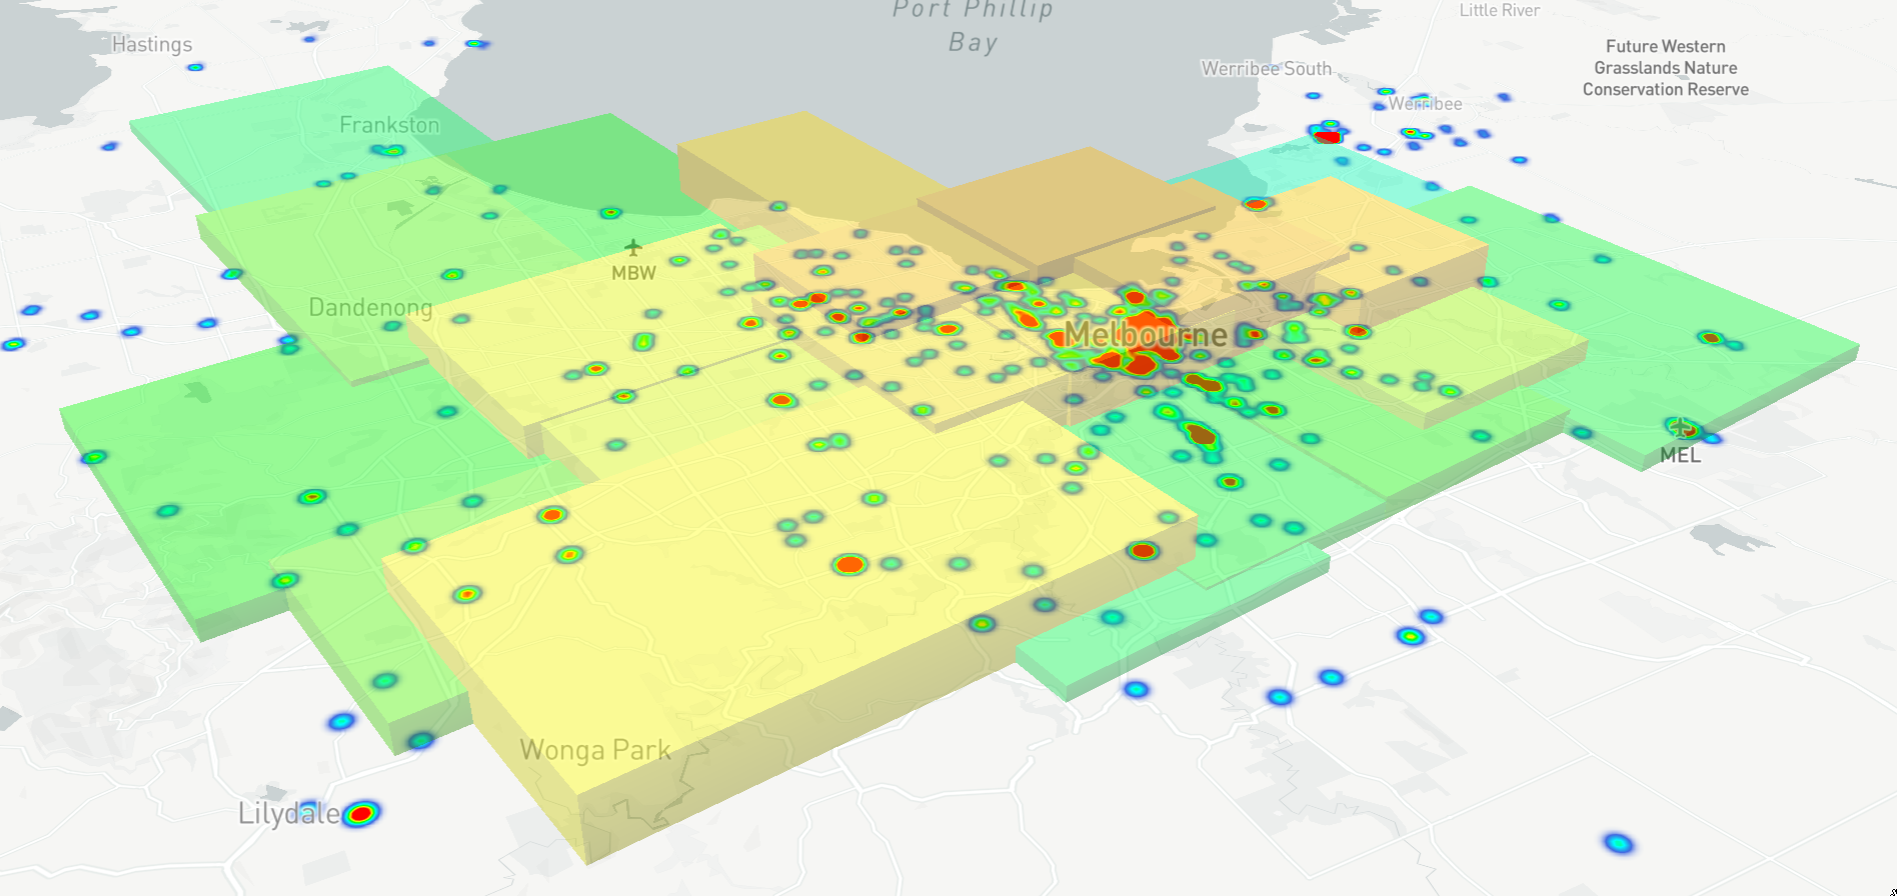
\includegraphics[width=12cm,keepaspectratio=true]{images/heatmap_visualisation.png}
    \caption{Visualisation of tweet density overlaid with obesity statistics.}
    \label{fig:visheatmap}
\end{figure}

\subsection{Data interactions}

As map features for both tweet and AURIN data contain metadata, they are able to be directly interacted with to learn more about the data, as seen in Figure \ref{fig:visinteract}.

\begin{figure}[H]
    \centering
    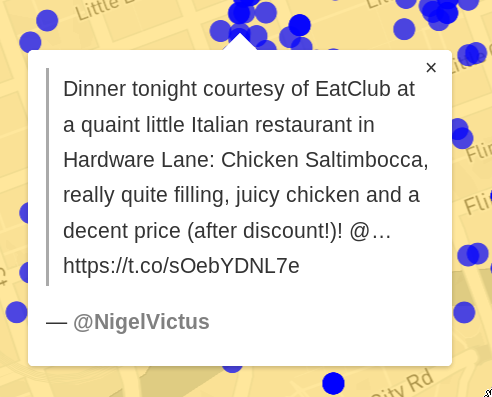
\includegraphics[width=8cm,keepaspectratio=true]{images/interact.png}
    \caption{Inspecting tweet data.}
    \label{fig:visinteract}
\end{figure}

\subsection{Exploring data} \label{explore}
This feature helps in providing in-depth analysis of the story using various visualizations. After tweets are plot on the map and corresponding data correlation set of AURIN is selected, user can use explore module to get more analysis from the data which is plotted on the map as shown in Figure \ref{fig:exploreui}.

\begin{figure}[H]
    \centering
    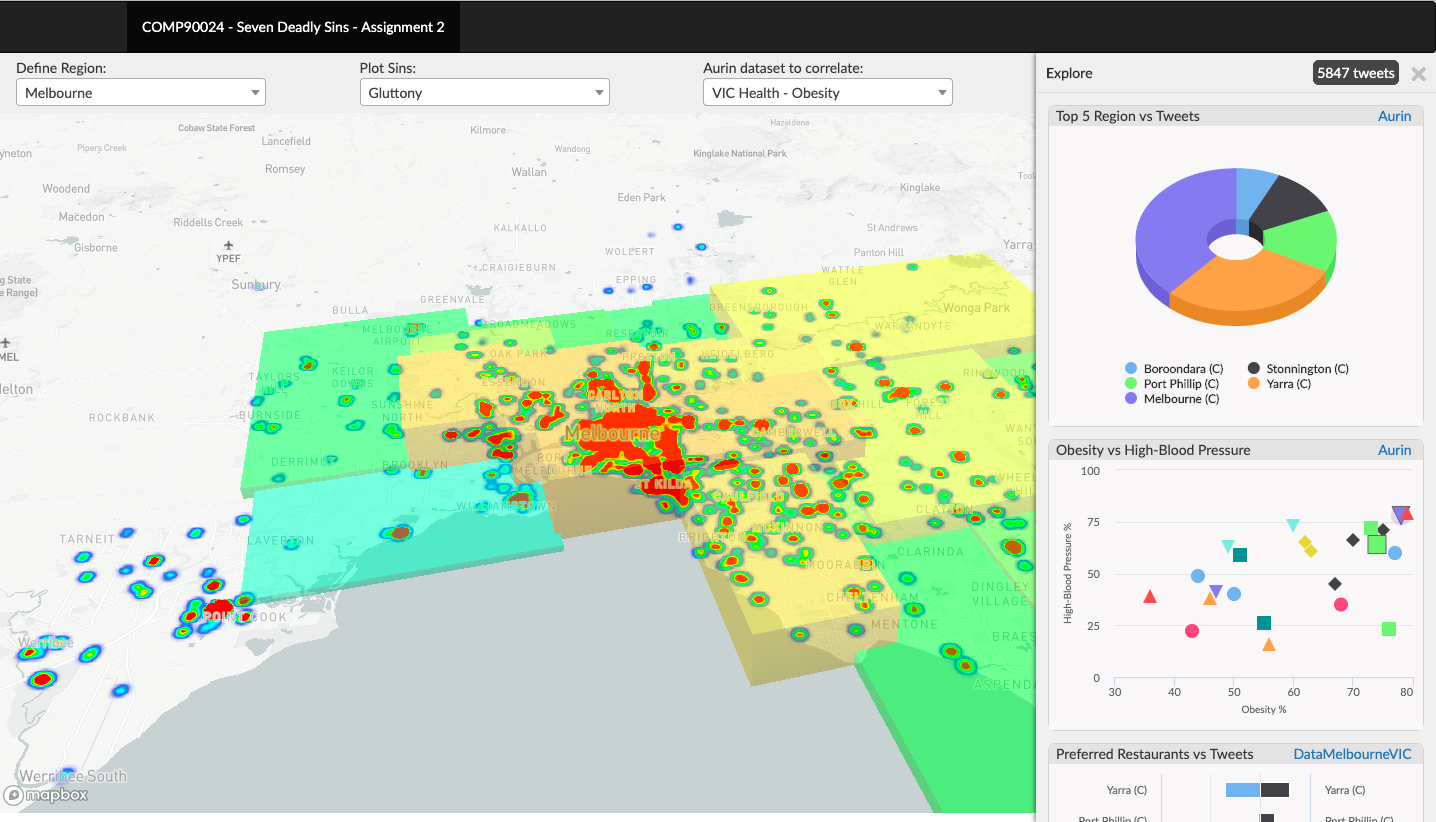
\includegraphics[width=10cm,keepaspectratio=true]{images/explore_UI.png}
    \caption{Exploring data for in-depth analysis}
    \label{fig:exploreui}
\end{figure}

It can be used while visualizing data on the map as it overlays on the top. The view helps in explaining different aspect of the data using pie-chart, scatter-plot and comparison multi-column bar-chart. The idea is to see how correlation of the AURIN dataset is working with the kind of tweets extracted from the users. A scenario of gluttony tweets with respect to AURIN correlation of health data using explore feature is shown in Figure \ref{fig:exploreui2}.

\begin{figure}[H]
    \centering
    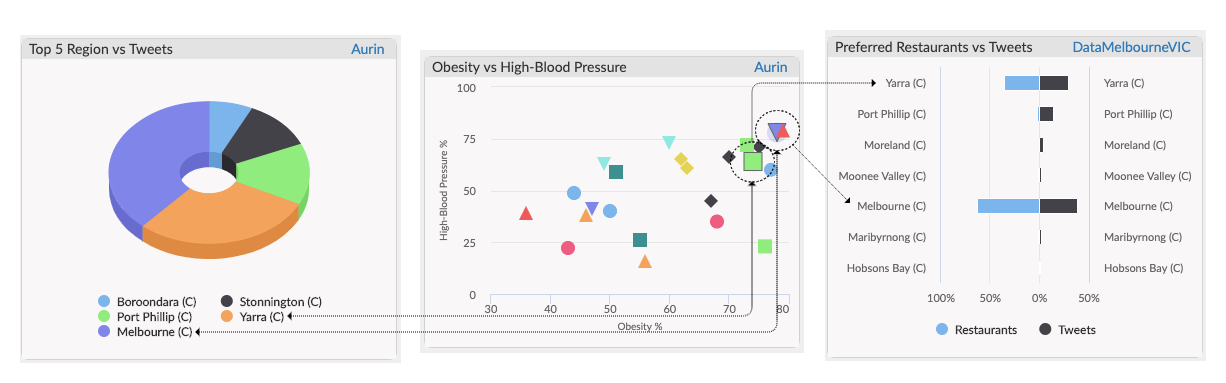
\includegraphics[width=16cm,keepaspectratio=true]{images/visualization_explore.png}
    \caption{Analyzing correlation of gluttony tweets with multiple data sources}
    \label{fig:exploreui2}
\end{figure}

Using multiple charts of the explore view, we can see how correlation is working with different data sources and tweets. As shown in the figure, \texttt{Melbourne} and \texttt{Yarra} are the regions where most of the gluttony tweets are found by the harvester using its analysis engine. Comparing this information with scatter plot, it is also noticed that these regions indeed have high patients of obesity and blood-pressure. Moreover, the assumption that these regions will then have higher number of preferred restaurants is also seen by using some other data source from DataMelbourneVic\footnote{https://data.melbourne.vic.gov.au/Economy/Cafes-and-restaurants-with-seating-capacity/xt2y-tnn9}. Hence, exploration of data with these visualization helped us to define a strong hypothesis for extracted gluttony tweets.
